\documentclass[11pt,a4paper]{article}
\usepackage[T1]{fontenc}
\usepackage[utf8]{inputenc}
\usepackage{lmodern}
\usepackage[a4paper,top=2.5cm,bottom=2.5cm,left=2.6cm,right=2.6cm,headheight=14pt]{geometry}
\usepackage{amsmath,amssymb,bm}
\usepackage{booktabs}
\usepackage{graphicx}
\usepackage{float}
\usepackage{enumitem}
\usepackage{array}
\usepackage{fancyhdr}
\usepackage[font=small,labelfont=bf,labelsep=colon]{caption}
\usepackage[hidelinks]{hyperref}

\graphicspath{{figures/}}

\pagestyle{fancy}
\fancyhf{}
\fancyhead[L]{\small Regression and Time Series Models}
\fancyhead[R]{\small ARIMA Modelling of the 10-Year Treasury Yield}
\fancyfoot[C]{\thepage}
\renewcommand{\headrulewidth}{0.5pt}

\setlist{itemsep=0.3em}

\begin{document}

%======================================================================
\begin{titlepage}
\centering
\vspace*{3cm}
{\large\textsc{Regression and Time Series Models}}\\[0.8em]
{\normalsize Master's Degree Programme -- Group Project}

\vspace{3.5cm}
\rule{\textwidth}{0.6pt}\\[1em]
{\LARGE\bfseries ARIMA Modelling of the 10-Year\\[0.3em] US Treasury Yield}\\[0.8em]
\rule{\textwidth}{0.6pt}

\vspace{3cm}
{\large\bfseries Group N members}\\[0.8em]
{\large Name Surname}\\[0.4em]
{\large Name Surname}\\[0.4em]
{\large Name Surname}

\vfill
{\large 26 November 2026}
\end{titlepage}

%======================================================================
\setcounter{page}{1}
\noindent\textbf{\large Declaration of AI Use}\\[0.3em]
We used AI tools to help review and extend the Python code, to draft parts of the explanations and to build and format the \LaTeX{} file. All numerical results come from running the project notebook, and the custom implementations of the tests and of the ARIMA estimator were cross-checked against the \texttt{statsmodels} library (Section~\ref{sec:check}). The authors reviewed the whole manuscript and take full responsibility for its content.

\newpage
\tableofcontents
\newpage

%======================================================================
\section{Introduction and dataset}

The goal of this project is to build and critically assess an ARIMA model for the 10-year US Treasury yield. Besides choosing the orders of the model, we want to check whether its assumptions hold (stationarity of the differenced series, white-noise residuals, stable parameters) and whether it forecasts better than the simplest benchmark for an interest rate, the random walk.

The data come from the FRED database of the Federal Reserve Bank of St.\ Louis.

\begin{table}[H]
\centering
\begin{tabular}{lll}
\toprule
Variable & Type & Description \\
\midrule
\texttt{date} & monthly & First day of the month, January 2000 -- October 2026 ($T = 322$) \\
\texttt{GS10} & continuous & 10-year Treasury constant-maturity yield (\%), \emph{response} $y_t$ \\
\bottomrule
\end{tabular}
\caption{Variables of the dataset.}
\end{table}

Each monthly value is the \emph{average of the daily yields} of the business days of the month. This detail turns out to be important for the choice of the model (Section~\ref{sec:ma1}). The yield starts at 6.66\% in January 2000, reaches its minimum of 0.62\% in July 2020 and ends at 5.13\%.

The analysis was carried out in Python with a custom implementation of the ADF and KPSS tests, of the ACF and PACF, of the ARMA estimator and of the diagnostic tests. The results were then double-checked with \texttt{statsmodels} (Section~\ref{sec:check}). Throughout, $y_t$ denotes the yield in percent and $\Delta y_t = y_t - y_{t-1}$ its monthly change in percentage points.

\begin{figure}[H]
\centering
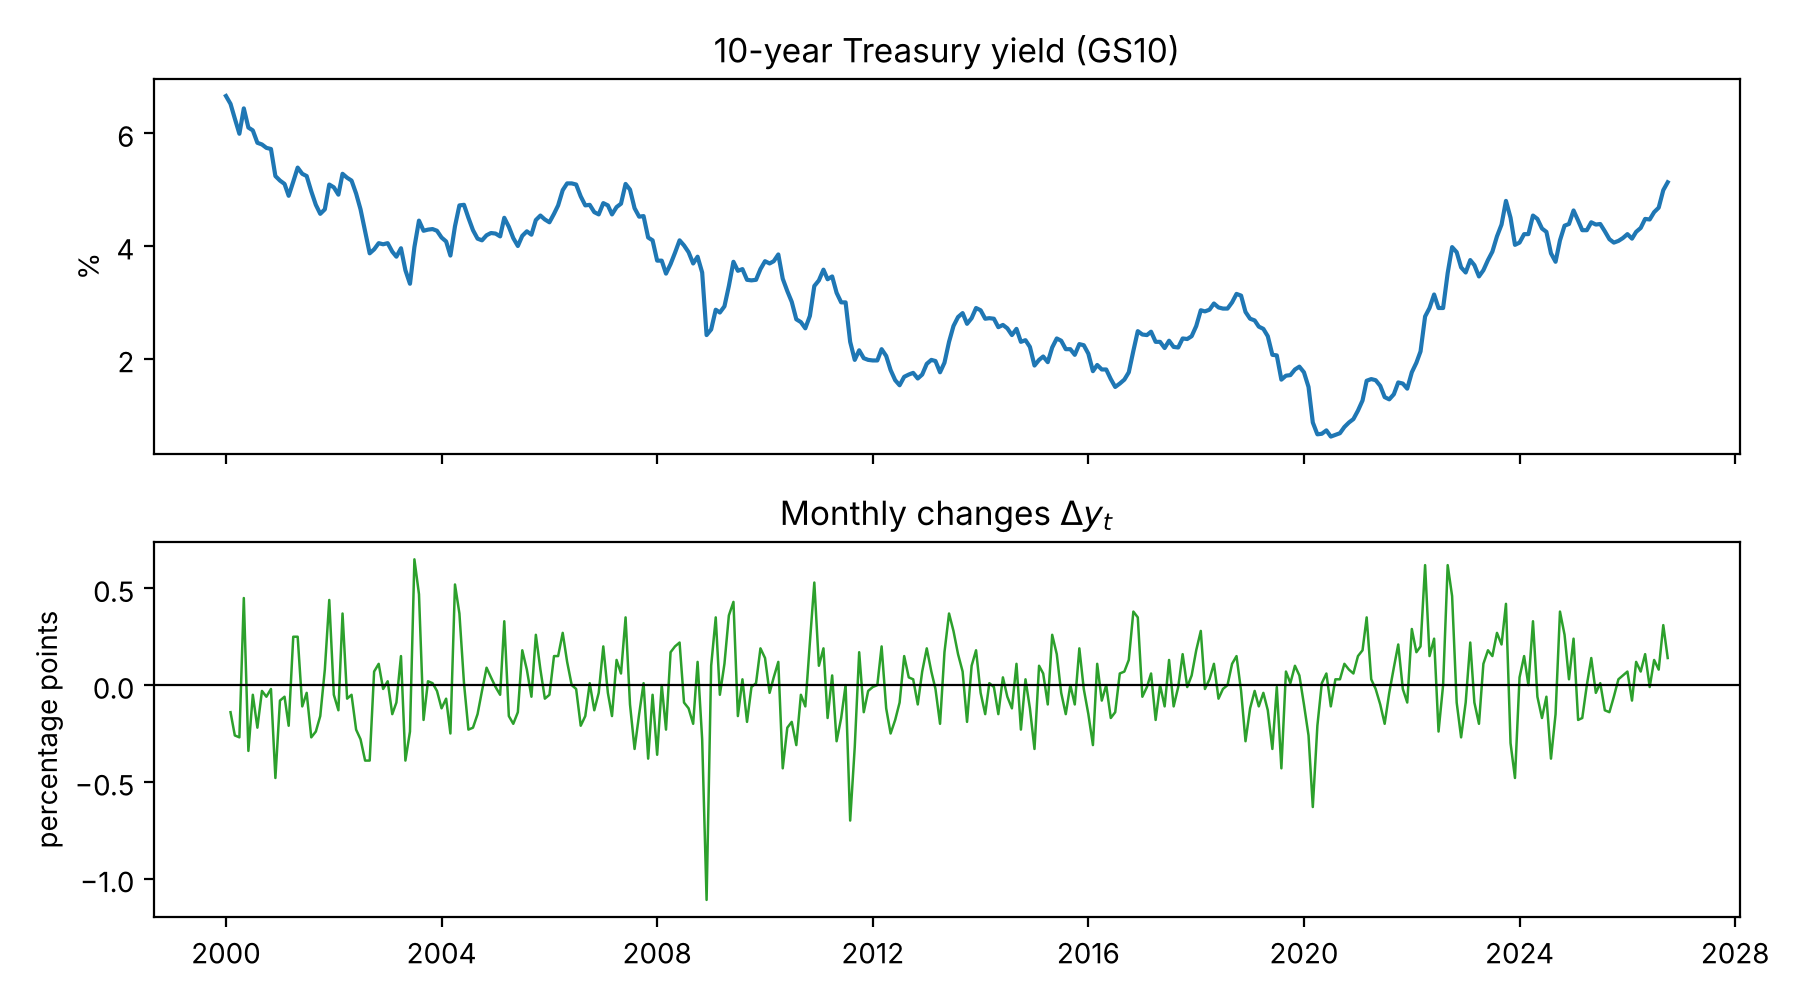
\includegraphics[width=0.85\textwidth]{series.png}
\caption{GS10 yield (top) and its monthly changes (bottom).}
\label{fig:series}
\end{figure}

%======================================================================
\section{Data transformation}

\subsection{Levels or logarithms}

GS10 is an interest rate, not a price. The log-difference $\Delta\log y_t$ is therefore not a return but the \emph{percentage change of the rate}: with the yield at 0.62\% a move of 0.1 points is a 16\% change, with the yield at 5\% it is a 2\% change. Since time-varying variance models (GARCH) are outside the scope of the course, we choose the transformation whose variance is more stable over time. Table~\ref{tab:var} compares the two candidate differenced series in four sub-periods.

\begin{table}[H]
\centering
\begin{tabular}{lccc}
\toprule
Period & Mean level (\%) & s.d.\ of $\Delta y_t$ (p.p.) & s.d.\ of $\Delta\log y_t$ \\
\midrule
2000--2007 & $4.69$ & $0.218$ & $0.049$ \\
2008--2014 & $2.80$ & $0.234$ & $0.085$ \\
2015--2021 & $1.96$ & $0.168$ & $0.108$ \\
2022--2026 & $3.97$ & $0.223$ & $0.067$ \\
\midrule
Max / min ratio & & $1.40$ & $2.23$ \\
\bottomrule
\end{tabular}
\caption{Standard deviation of the monthly changes by sub-period.}
\label{tab:var}
\end{table}

\textbf{Result.} In percentage points the standard deviation stays between roughly 0.17 and 0.23 in every sub-period, whereas in logarithms it more than doubles in the years of near-zero rates (Figure~\ref{fig:rolling}). \textbf{We therefore model the yield in levels.}

\begin{figure}[H]
\centering
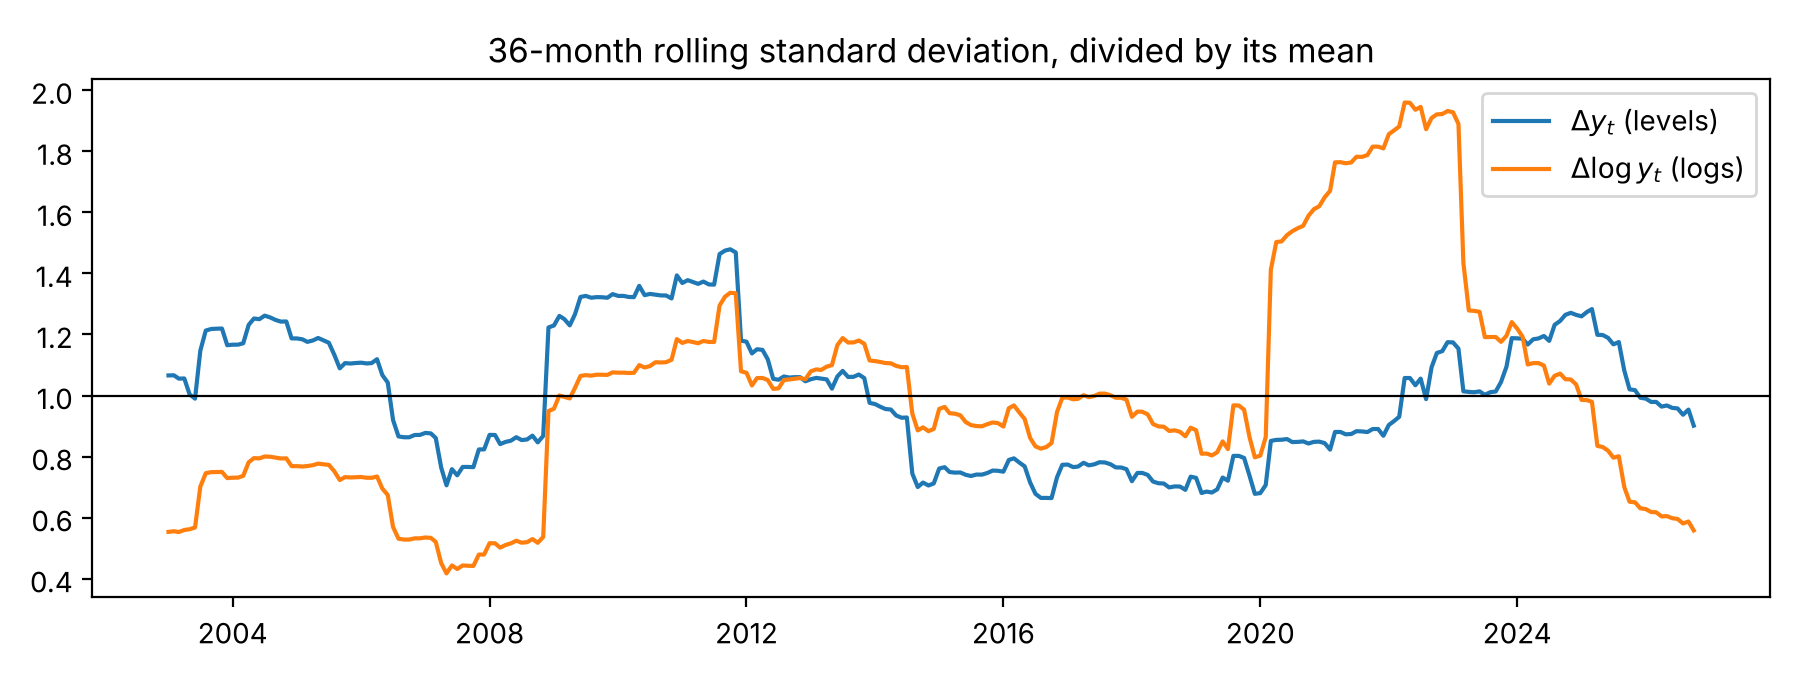
\includegraphics[width=0.85\textwidth]{rolling_sd.png}
\caption{36-month rolling standard deviation of the two differenced series, divided by its mean. The log-changes amplify volatility when rates are low.}
\label{fig:rolling}
\end{figure}

\subsection{Distribution of the monthly changes}

The monthly changes have mean $-0.0048$, standard deviation $0.213$, skewness $-0.22$ and kurtosis $5.45$. The kurtosis well above 3 indicates tails heavier than the normal ones (extreme months such as late 2008 and 2022), which will matter when judging the forecast intervals.

\begin{figure}[H]
\centering
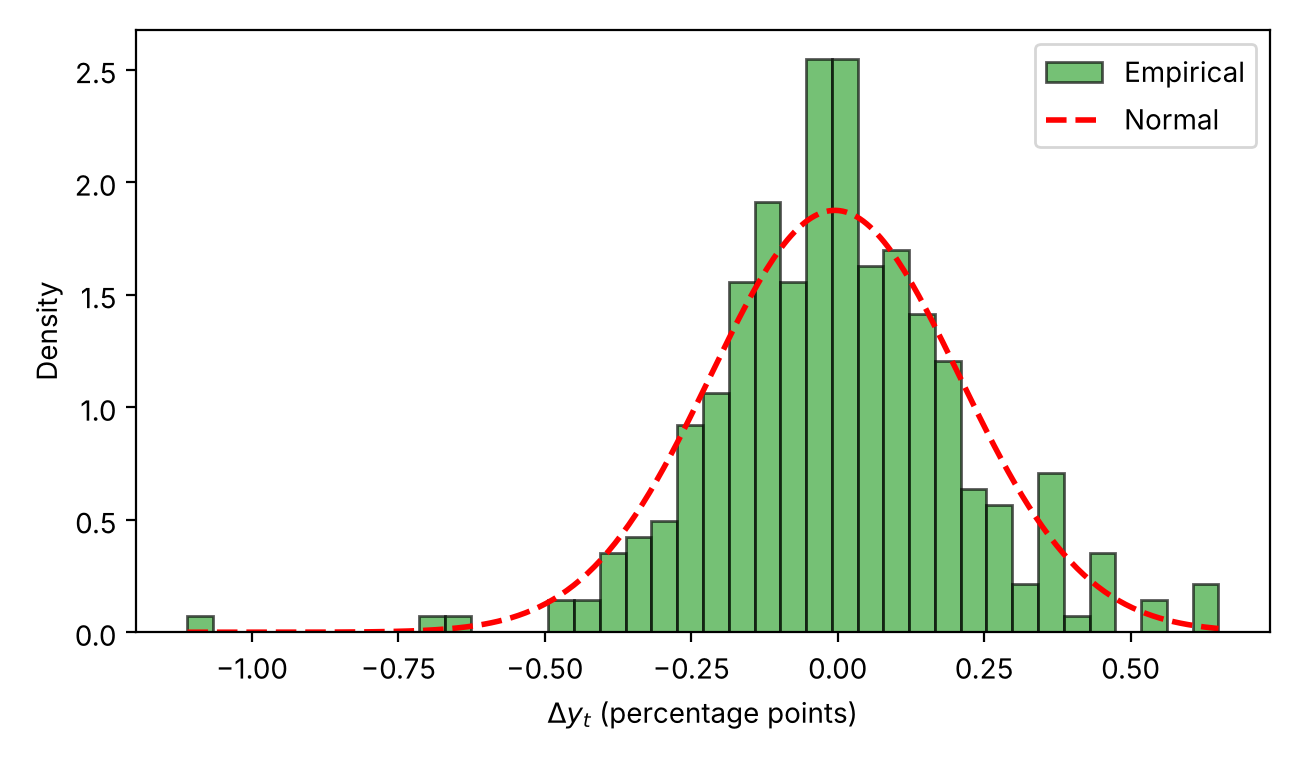
\includegraphics[width=0.6\textwidth]{distribution.png}
\caption{Histogram of $\Delta y_t$ with the normal density with the same mean and variance.}
\end{figure}

%======================================================================
\section{Stationarity and order of integration}

\subsection{Why the ADF and KPSS tests together}

The two tests have reversed hypotheses, and each keeps its null until the data contradict it. When they agree the conclusion is robust.

\textbf{Augmented Dickey--Fuller.} The test regression is
\begin{equation}
\Delta y_t = \alpha \,(+\, \beta t) + \delta\, y_{t-1} + \sum_{j=1}^{p}\gamma_j \Delta y_{t-j} + e_t,
\end{equation}
with $H_0: \delta = 0$ (unit root) against $H_1: \delta < 0$ (stationarity). The statistic is $\tau = \hat\delta/SE(\hat\delta)$, with the OLS standard error. Under $H_0$ it does not follow a $t$ distribution, so it is compared with the Dickey--Fuller critical values (MacKinnon response surfaces for the actual sample size) and $H_0$ is rejected in the \emph{left} tail. The number of lags $p$ is chosen by AIC, with all candidate regressions estimated on the same observations.

\textbf{KPSS.} With $\hat e_t$ the residuals of $y_t$ on a constant (or on a constant and a trend) and $S_t = \sum_{s\le t}\hat e_s$ their partial sums,
\begin{equation}
\eta = \frac{\sum_{t=1}^{T} S_t^2}{T^2\,\hat\sigma^2_{LR}}, \qquad \hat\sigma^2_{LR} = \hat\gamma_0 + 2\sum_{j=1}^{L}\Big(1 - \frac{j}{L+1}\Big)\hat\gamma_j,
\end{equation}
with $H_0$: stationarity, rejected in the \emph{right} tail, and $L = \lfloor 4(T/100)^{1/4}\rfloor$.

\textbf{Which version.} On the levels we use both the version with a constant (\texttt{'c'}) and the one with a constant and a linear trend (\texttt{'ct'}), because the yield falls for twenty years and then rises. On the differences we use only \texttt{'c'}: a linear trend in the levels would become a constant in the differences.

\subsection{Results}

\begin{table}[H]
\centering
\small
\begin{tabular}{llcccl|ccl}
\toprule
Series & Version & ADF $\tau$ & lags & 5\% crit. & ADF & KPSS $\eta$ & 5\% crit. & KPSS \\
\midrule
$y_t$ & \texttt{'c'} & $-2.19$ & 2 & $-2.87$ & unit root & $2.073$ & $0.463$ & non-stationary \\
$y_t$ & \texttt{'ct'} & $-1.45$ & 2 & $-3.42$ & unit root & $0.862$ & $0.146$ & non-stationary \\
$\Delta y_t$ & \texttt{'c'} & $-12.36$ & 1 & $-2.87$ & stationary & $0.420$ & $0.463$ & stationary \\
\bottomrule
\end{tabular}
\caption{Stationarity tests. ADF: reject if $\tau$ is below the critical value. KPSS: reject if $\eta$ is above it.}
\end{table}

In both versions the ADF does not reject the unit root in the levels and the KPSS rejects their stationarity: \textbf{the yield is non-stationary}. On the differences the ADF strongly rejects the unit root and the KPSS does not reject stationarity: \textbf{the monthly changes are stationary}. Hence $d = 1$.

\subsection{Drift}

With $d = 1$ the constant of the model is the drift, i.e.\ the mean monthly change. We test $H_0$: $\mathbb{E}[\Delta y_t] = 0$ with Newey--West standard errors, $SE = \sqrt{\hat\sigma^2_{LR}/T}$, since $\Delta y_t$ is autocorrelated.

\textbf{Result.} The estimated drift is $-0.0048$ points per month, with $t = -0.36$ and $p = 0.72$: \textbf{no significant drift}, so the model has no constant.

Note that the $t$-test on a trend in the levels, $y_t = a + bt + u_t$, would give $t = -3.41$, apparently significant. With a unit root, however, that statistic is not normally distributed and is inflated (spurious regression). This is why, once the ADF has not rejected, the drift is tested on the differences.

%======================================================================
\section{Is there anything to model?}

If $\Delta y_t$ were white noise the best forecast would be the random walk, $\hat y_{T+1} = y_T$, and no ARMA model would be needed. We use the Ljung--Box test,
\begin{equation}
Q = T(T+2)\sum_{k=1}^{m}\frac{\hat\rho_k^2}{T-k} \;\sim\; \chi^2_{m} \ \text{under } H_0,
\end{equation}
with $m$ degrees of freedom because no ARMA parameter has been estimated yet.

\begin{table}[H]
\centering
\begin{tabular}{cccccl}
\toprule
$m$ & d.f. & $Q$ & 5\% crit. & $p$-value & Decision (5\%) \\
\midrule
6 & 6 & $22.76$ & $12.59$ & $< 0.001$ & reject $H_0$ \\
12 & 12 & $27.45$ & $21.03$ & $0.0067$ & reject $H_0$ \\
\bottomrule
\end{tabular}
\caption{Ljung--Box test on the monthly changes.}
\end{table}

The test rejects: the monthly changes are autocorrelated. The Durbin--Watson statistic of the random-walk residuals, which are exactly the $\Delta y_t$, is $1.514$, i.e.\ $\hat\rho_1 \approx 1 - d/2 = 0.24$.

%======================================================================
\section{Identification}

\subsection{ACF and PACF}

For the ACF we use Bartlett bands: at lag $k$ the band is $\pm 1.96\sqrt{(1 + 2\sum_{j<k}\hat\rho_j^2)/T}$, which tests $H_0$: MA($k-1$). For the PACF the band is $\pm 1.96/\sqrt{T} = \pm0.109$, which tests $H_0$: AR($k-1$). The suggested order is the \emph{first non-significant lag minus one}, i.e.\ the point where the function cuts off.

\begin{figure}[H]
\centering
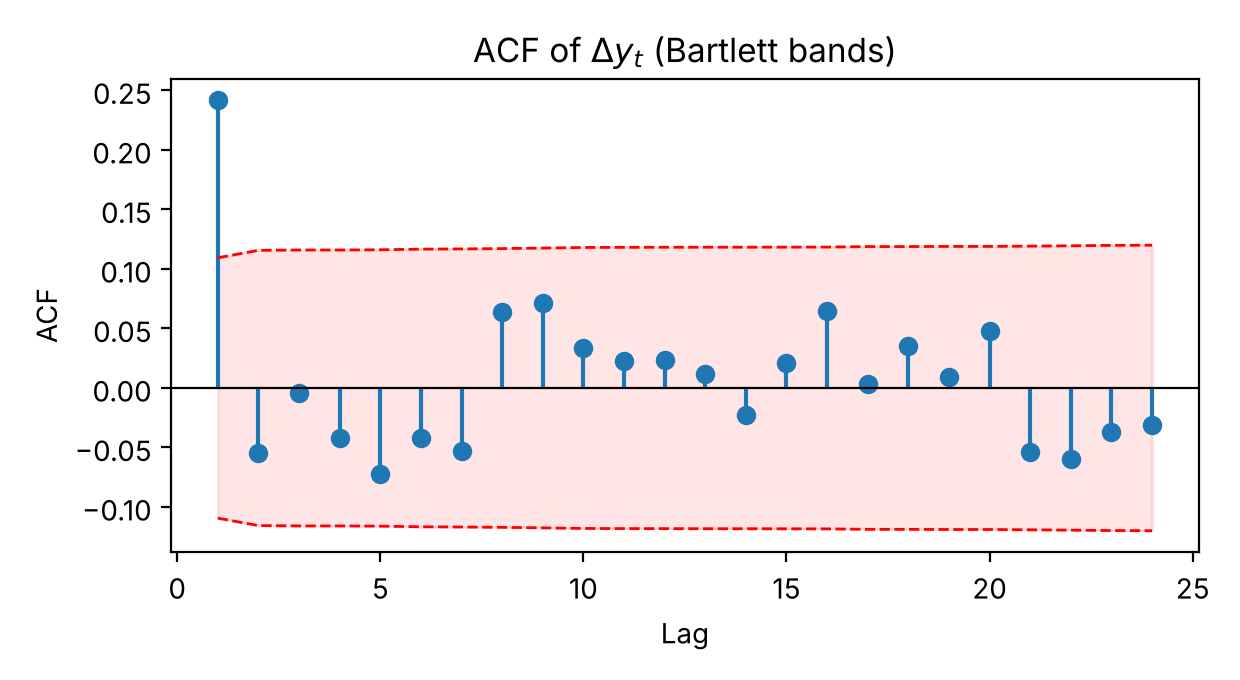
\includegraphics[width=0.49\textwidth]{acf_dy.png}\hfill
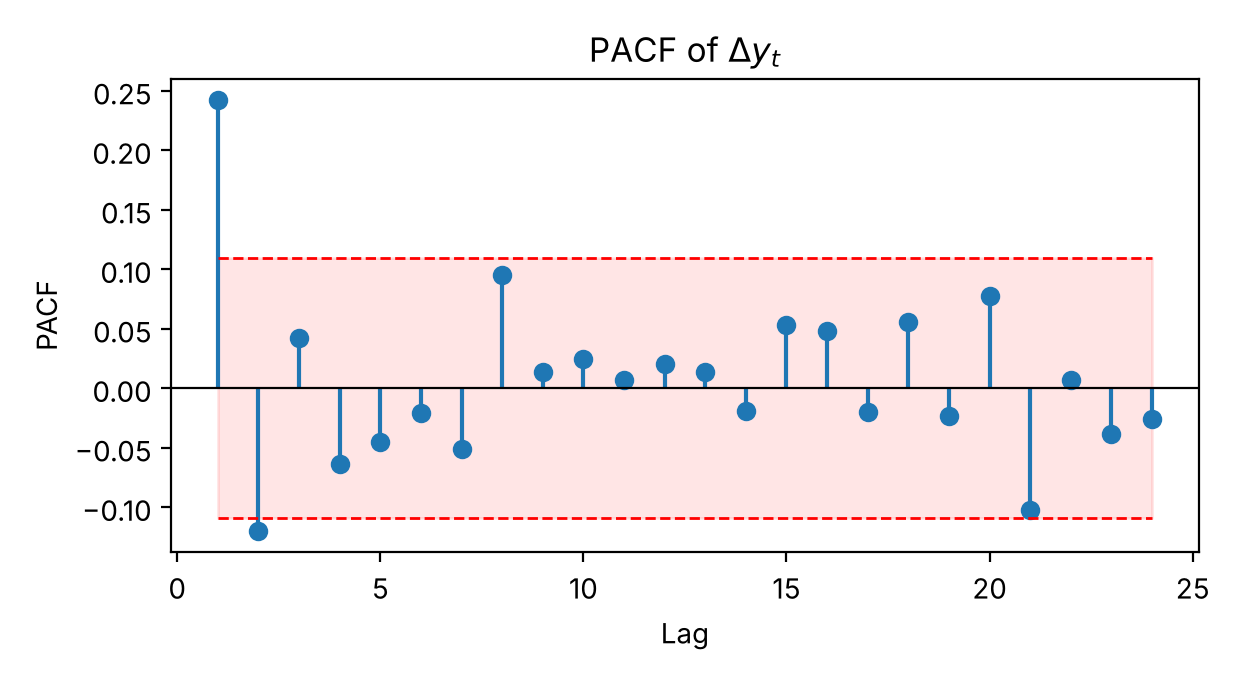
\includegraphics[width=0.49\textwidth]{pacf_dy.png}
\caption{ACF with Bartlett bands (left) and PACF (right) of $\Delta y_t$.}
\end{figure}

\begin{table}[H]
\centering
\begin{tabular}{lcccccc}
\toprule
Lag & 1 & 2 & 3 & 4 & 5 & 6 \\
\midrule
ACF & $0.242$ & $-0.055$ & $-0.004$ & $-0.042$ & $-0.072$ & $-0.042$ \\
PACF & $0.242$ & $-0.120$ & $0.042$ & $-0.064$ & $-0.045$ & $-0.021$ \\
\bottomrule
\end{tabular}
\caption{Sample autocorrelations of $\Delta y_t$.}
\end{table}

\textbf{Interpretation.} The ACF has a single significant bar at lag 1 and then cuts off: the signature of an \textbf{MA(1)}. The PACF decays with alternating sign ($0.24$, then $-0.12$), as in an MA(1) with $\theta > 0$; taken literally it also suggests an AR(2). Moreover $\hat\rho_1 > 0$, so the series is not over-differenced (an unnecessary difference would give $\hat\rho_1$ close to $-0.5$).

\textbf{Why not ``the last significant lag''.} Looking at 20 lags, each with a 5\% probability of falling outside the bands by chance, the probability that at least one does is $1 - 0.95^{20} \approx 64\%$. Choosing the last significant lag would therefore pick a spurious order; in a first version of our code this rule selected a random bar at lag 15 and an ARMA(15,\,1).

\subsection{Where the MA(1) comes from}\label{sec:ma1}

Suppose the \emph{daily} yield is a random walk, $x_s = x_{s-1} + u_s$, with independent shocks of variance $\sigma_u^2$, and that the monthly figure is the average over the $M$ business days of the month, $A_k = \frac{1}{M}\sum_{i=1}^{M} x_{(k-1)M+i}$.

The shock of day $i$ of month $k$ moves all subsequent values. It enters the average of month $k$ on $M - i + 1$ days out of $M$, and the average of month $k+1$ on all days. Its weight is therefore $(M-i+1)/M$ in $\Delta A_k$ and $(i-1)/M$ in $\Delta A_{k+1}$. The two consecutive changes share only the shocks of month $k$, so, with $j = i - 1$,
\begin{align}
\mathrm{Cov}(\Delta A_k, \Delta A_{k+1}) &= \frac{\sigma_u^2}{M^2}\sum_{j=0}^{M-1}(M-j)\,j = \frac{\sigma_u^2}{M^2}\cdot\frac{M(M^2-1)}{6},\\
\mathrm{Var}(\Delta A_k) &= \frac{\sigma_u^2}{M^2}\Big[\sum_{j=0}^{M-1} j^2 + \sum_{j=1}^{M} j^2\Big] = \frac{\sigma_u^2}{M^2}\cdot\frac{M(4M^2+2)}{6},
\end{align}
and
\begin{equation}
\rho_1 = \frac{M^2-1}{2(2M^2+1)} \;\xrightarrow{M\to\infty}\; \frac14, \qquad \rho_k = 0 \ \text{ for } k \ge 2,
\end{equation}
because changes two months apart share no shock (Working, 1960). With $M = 21$ business days $\rho_1 = 0.249$, very close to the observed $\hat\rho_1 = 0.242$. An autocorrelation at lag 1 only is exactly an MA(1), whose coefficient solves
\begin{equation}
\frac{\theta}{1+\theta^2} = \frac14 \;\Longrightarrow\; \theta^2 - 4\theta + 1 = 0 \;\Longrightarrow\; \theta = 2 - \sqrt{3} \approx 0.268.
\end{equation}

%======================================================================
\section{Order selection}

We estimate all ARMA($p$, $q$) models for $\Delta y_t$ with $p, q \le 3$ and no constant, plus the ARMA(15,\,1) suggested by the last-significant-lag rule, and compare them \emph{on the same observations} (the first 16 are discarded):
\begin{equation}
\mathrm{AIC} = \log\frac{\mathrm{RSS}}{n} + \frac{2k}{n}, \qquad \mathrm{BIC} = \log\frac{\mathrm{RSS}}{n} + \frac{k\log n}{n}.
\end{equation}

\begin{table}[H]
\centering
\begin{tabular}{lccc}
\toprule
Model for $\Delta y_t$ & $k$ & AIC & BIC \\
\midrule
ARMA(0,\,1) & 1 & $-3.1951$ & $-3.1829$ \\
ARMA(0,\,2) & 2 & $-3.1942$ & $-3.1698$ \\
ARMA(1,\,1) & 2 & $-3.1883$ & $-3.1639$ \\
ARMA(2,\,0) & 2 & $-3.1879$ & $-3.1635$ \\
ARMA(1,\,0) & 1 & $-3.1745$ & $-3.1623$ \\
ARMA(1,\,2) & 3 & $-3.1884$ & $-3.1518$ \\
\midrule
ARMA(15,\,1) & 16 & $-3.1201$ & $-2.9250$ \\
\bottomrule
\end{tabular}
\caption{The six models with the lowest BIC and the ARMA(15,\,1), which ranks 17th out of 17.}
\end{table}

The \textbf{MA(1)} has both the lowest BIC and the lowest AIC. The neighbouring models add a parameter without improving the fit enough, and the ARMA(15,\,1) uses 16 parameters to describe what a single $\theta$ already captures. The selected model is
\begin{equation}
\Delta y_t = \varepsilon_t + \theta\,\varepsilon_{t-1}, \qquad \text{i.e.\ an ARIMA(0,\,1,\,1) without constant.}
\end{equation}

%======================================================================
\section{Estimation}

\subsection{Hannan--Rissanen estimator}

The lagged shock $\varepsilon_{t-1}$ is not observed, so $\theta$ cannot be estimated by a direct OLS regression. We proceed in two OLS steps:
\begin{enumerate}
\item a long autoregression of order $\lfloor(\log T)^2\rfloor$ is fitted and its residuals $\tilde\varepsilon_t$ are taken as estimates of the shocks;
\item $\Delta y_t$ is regressed on $\tilde\varepsilon_{t-1}$, and the standard error comes from $\hat\sigma^2(\mathbf{X}'\mathbf{X})^{-1}$ of this second regression.
\end{enumerate}
The shocks of the final model are then rebuilt recursively, $\hat\varepsilon_t = \Delta y_t - \hat\theta\,\hat\varepsilon_{t-1}$.

\subsection{Estimated parameter}

\begin{table}[H]
\centering
\begin{tabular}{lccccl}
\toprule
Parameter & Estimate & Std.\ error & $t$ & $p$-value & Decision (5\%) \\
\midrule
$\theta$ & 0.3053 & 0.0621 & 4.92 & $< 0.001$ & reject $H_0$ \\
\bottomrule
\end{tabular}
\caption{Estimate of the ARIMA(0,\,1,\,1); $\hat\sigma = 0.2054$ percentage points.}
\end{table}

\textbf{Interpretation.} $\hat\theta$ is highly significant: about 31\% of each monthly shock is carried over to the following month's change. The root of $1 + \hat\theta z$ has modulus 3.28 $> 1$, so the model is \textbf{invertible}: past shocks can be recovered from the data and the representation is unique.

\textbf{Test of the averaging effect.} We test $H_0: \theta = 2 - \sqrt3 = 0.2679$ with $z = (\hat\theta - \theta_0)/SE(\hat\theta) = 0.60$, $p = 0.55$: the null is \textbf{not rejected}. The estimated dynamics are compatible with those produced by monthly averaging of a daily random walk alone.

%======================================================================
\section{Diagnostic checks}

\subsection{Residual autocorrelation}

If the model is correct, its residuals are white noise. The Ljung--Box test on the residuals has $m - p - q = m - 1$ degrees of freedom: the estimated parameter makes the residuals ``whiter'' than chance and uses up one degree of freedom.

\begin{table}[H]
\centering
\begin{tabular}{cccccl}
\toprule
$m$ & d.f. & $Q$ & 5\% crit. & $p$-value & Decision (5\%) \\
\midrule
6 & 5 & $2.98$ & $11.07$ & $0.7036$ & do not reject $H_0$ \\
12 & 11 & $7.07$ & $19.68$ & $0.7932$ & do not reject $H_0$ \\
24 & 23 & $13.95$ & $35.17$ & $0.9282$ & do not reject $H_0$ \\
\bottomrule
\end{tabular}
\caption{Ljung--Box test on the ARIMA(0,\,1,\,1) residuals.}
\end{table}

No rejection for $m = 6, 12, 24$, and no bar of the residual ACF exceeds $0.071$ in absolute value (Figure~\ref{fig:resacf}). A single parameter removes the autocorrelation of $\Delta y_t$: the Durbin--Watson statistic goes from $1.51$ to $2.05$. The Durbin--Watson test is reported only as an indication, because it is not valid for models with estimated dynamics; the Ljung--Box test is the formal check.

\begin{figure}[H]
\centering
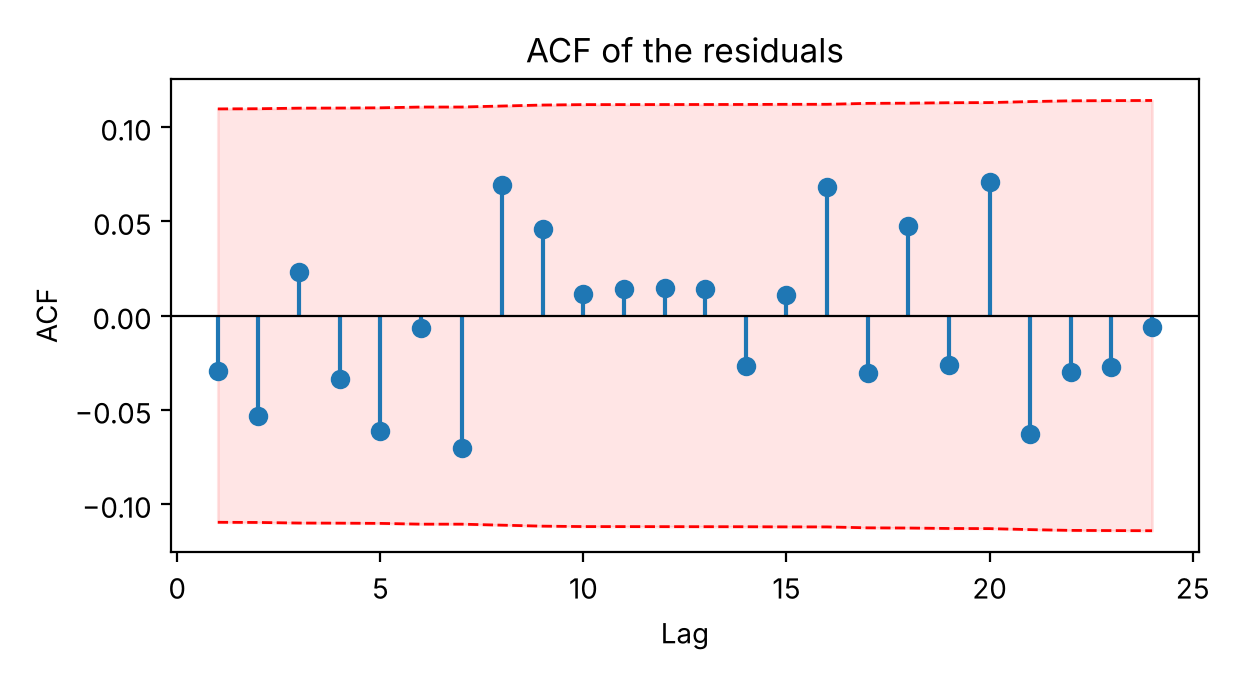
\includegraphics[width=0.6\textwidth]{acf_residuals.png}
\caption{ACF of the residuals with Bartlett bands.}
\label{fig:resacf}
\end{figure}

\subsection{Normality}

The Jarque--Bera statistic is
\begin{equation}
\mathrm{JB} = \frac{T}{6}\Big(S^2 + \frac{(K-3)^2}{4}\Big) \;\sim\; \chi^2_2 \ \text{under } H_0,
\end{equation}
with $S$ and $K$ the skewness and kurtosis of the residuals.

\textbf{Result.}
\begin{center}
\begin{tabular}{lc}
\toprule
Jarque--Bera test & Value \\
\midrule
$S$ & $-0.242$ \\
$K$ & 5.145 \\
JB & 64.48 \\
$p$-value & $< 0.001$ \\
Decision (5\%) & reject $H_0$ \\
\bottomrule
\end{tabular}
\end{center}

Normality is rejected because of the heavy tails, visible at the ends of the Q--Q plot (Figure~\ref{fig:res}). Point estimates and point forecasts remain valid; the normal-based 95\% intervals may be too narrow in extreme months, and their actual coverage is checked out of sample in Section~\ref{sec:oos}.

\begin{figure}[H]
\centering
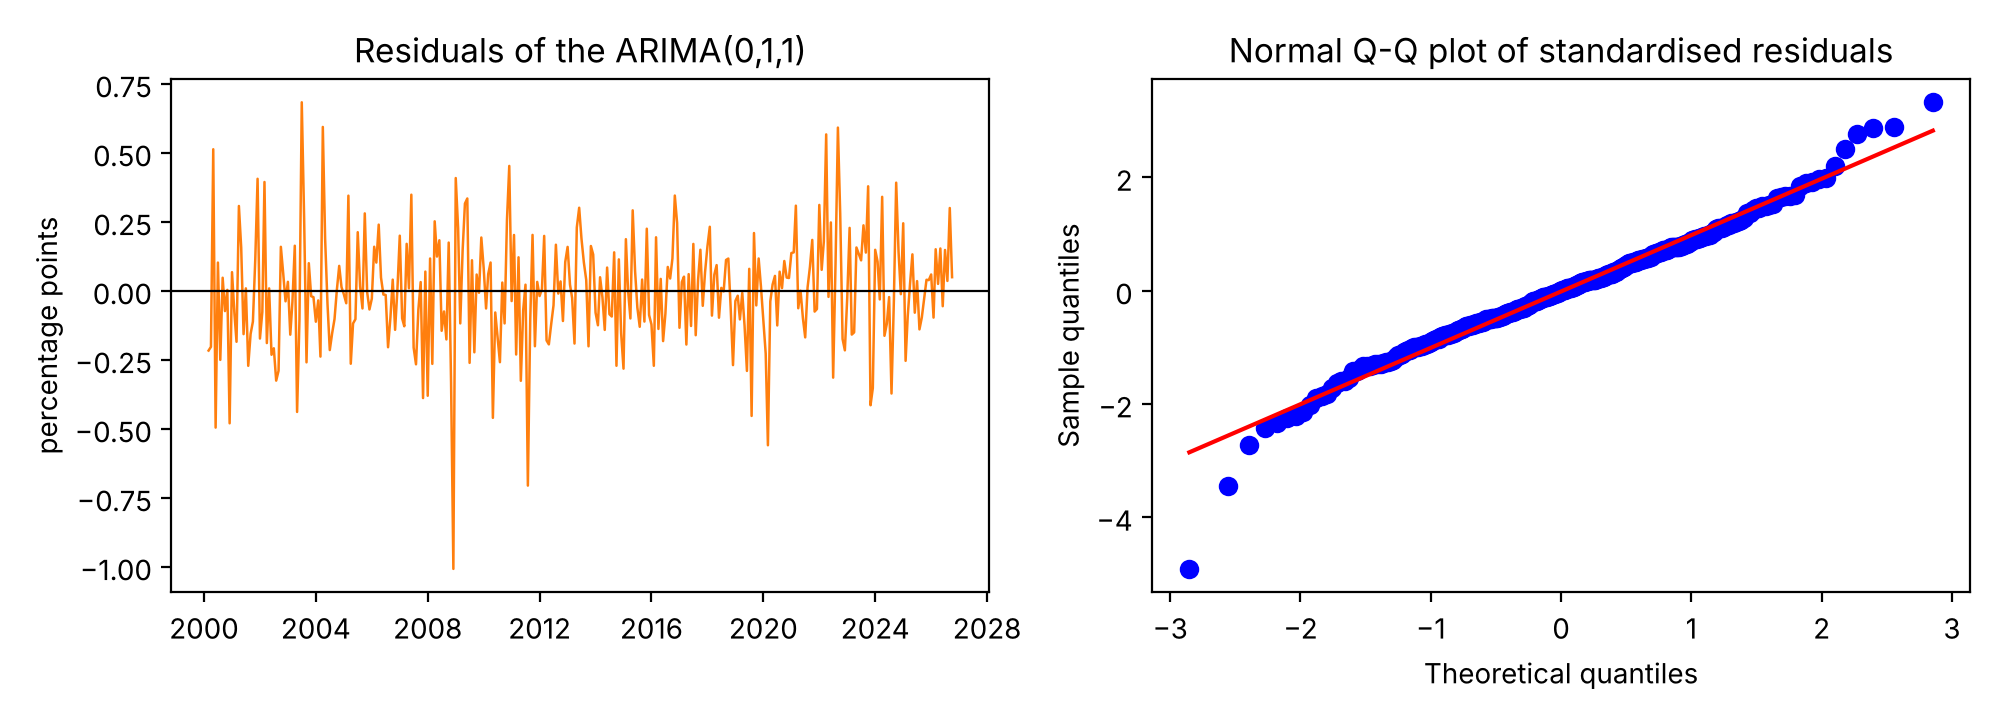
\includegraphics[width=0.95\textwidth]{residuals.png}
\caption{Residuals over time (left) and normal Q--Q plot of the standardised residuals (right).}
\label{fig:res}
\end{figure}

\subsection{Parameter stability}

We estimate the model separately on the two halves of the sample and compare the coefficients with $z = (\hat\theta_1 - \hat\theta_2)/\sqrt{SE_1^2 + SE_2^2}$.

\begin{table}[H]
\centering
\begin{tabular}{lcc}
\toprule
Sub-sample & $\hat\theta$ & Std.\ error \\
\midrule
January 2000 -- May 2013 & 0.247 & 0.096 \\
June 2013 -- October 2026 & 0.298 & 0.099 \\
\midrule
Difference & $z = -0.37$ & $p = 0.71$ \\
\bottomrule
\end{tabular}
\caption{Stability of $\theta$ across the two halves of the sample.}
\end{table}

The difference is not significant: $\theta$ is \textbf{stable} across very different regimes (the 2008 crisis, near-zero rates, the 2022 tightening). This is consistent with Section~\ref{sec:ma1}: the MA(1) depends on how the data are built (monthly averages), not on the phase of the cycle.

%======================================================================
\section{Forecast evaluation}

\subsection{Out-of-sample comparison}\label{sec:oos}

The last 64 observations (20\% of the sample, from July 2021, a period that includes the 2022 rise in rates) are forecast \emph{one step ahead with a rolling origin}: for every month the model is re-estimated on all previous data. We compare the forecasts with
\begin{equation}
\mathrm{RMSE} = \sqrt{\frac{1}{n}\sum_t e_t^2}, \qquad \mathrm{MAE} = \frac{1}{n}\sum_t |e_t|,
\end{equation}
with the \emph{coverage} of the 95\% intervals (share of actual values inside the interval) and with the Diebold--Mariano test,
\begin{equation}
d_t = e_{1,t}^2 - e_{2,t}^2, \qquad \mathrm{DM} = \frac{\bar d}{\sqrt{\hat\sigma^2_{LR}(d)/n}} \;\sim\; N(0,1),
\end{equation}
where $H_0$ is equal expected squared error and $\mathrm{DM} < 0$ means that model 1 forecasts better.

\begin{table}[H]
\centering
\begin{tabular}{lcccc}
\toprule
Model & RMSE & MAE & 95\% coverage & RMSE / RMSE RW \\
\midrule
\textbf{ARIMA(0,\,1,\,1)} & \textbf{0.2086} & \textbf{0.1616} & \textbf{95.3\%} & \textbf{0.938} \\
ARIMA(2,\,1,\,0) & 0.2087 & 0.1610 & 96.9\% & 0.938 \\
ARIMA(1,\,1,\,1) & 0.2093 & 0.1622 & 95.3\% & 0.941 \\
ARIMA(15,\,1,\,1) & 0.2188 & 0.1676 & 93.8\% & 0.984 \\
Random walk & 0.2225 & 0.1733 & 93.8\% & 1.000 \\
Random walk with drift & 0.2262 & 0.1758 & 92.2\% & 1.017 \\
\bottomrule
\end{tabular}
\caption{One-step-ahead out-of-sample forecasts (64 months).}
\end{table}

\textbf{Findings.}
\begin{itemize}
\item The ARIMA(0,\,1,\,1) has the lowest RMSE, about \textbf{6\% below the random walk}. Diebold--Mariano gives $\mathrm{DM} = -1.78$, one-sided $p = 0.038$ (two-sided $p = 0.075$). The gain is modest, as expected for a market interest rate, but systematic.
\item The ARIMA(2,\,1,\,0) and ARIMA(1,\,1,\,1) forecast almost equally well: they describe the same one-lag dynamics with one extra parameter.
\item The ARIMA(15,\,1,\,1) forecasts worse than the MA(1) ($\mathrm{DM} = -1.93$, one-sided $p = 0.027$): the extra parameters fit sample noise (\textbf{overfitting}).
\item Adding a drift worsens the random walk, consistently with the non-significant drift of Section 3.
\item The coverage of the ARIMA(0,\,1,\,1) intervals is 95.3\%: despite the heavy tails, the one-step intervals are reliable.
\end{itemize}

\begin{figure}[H]
\centering
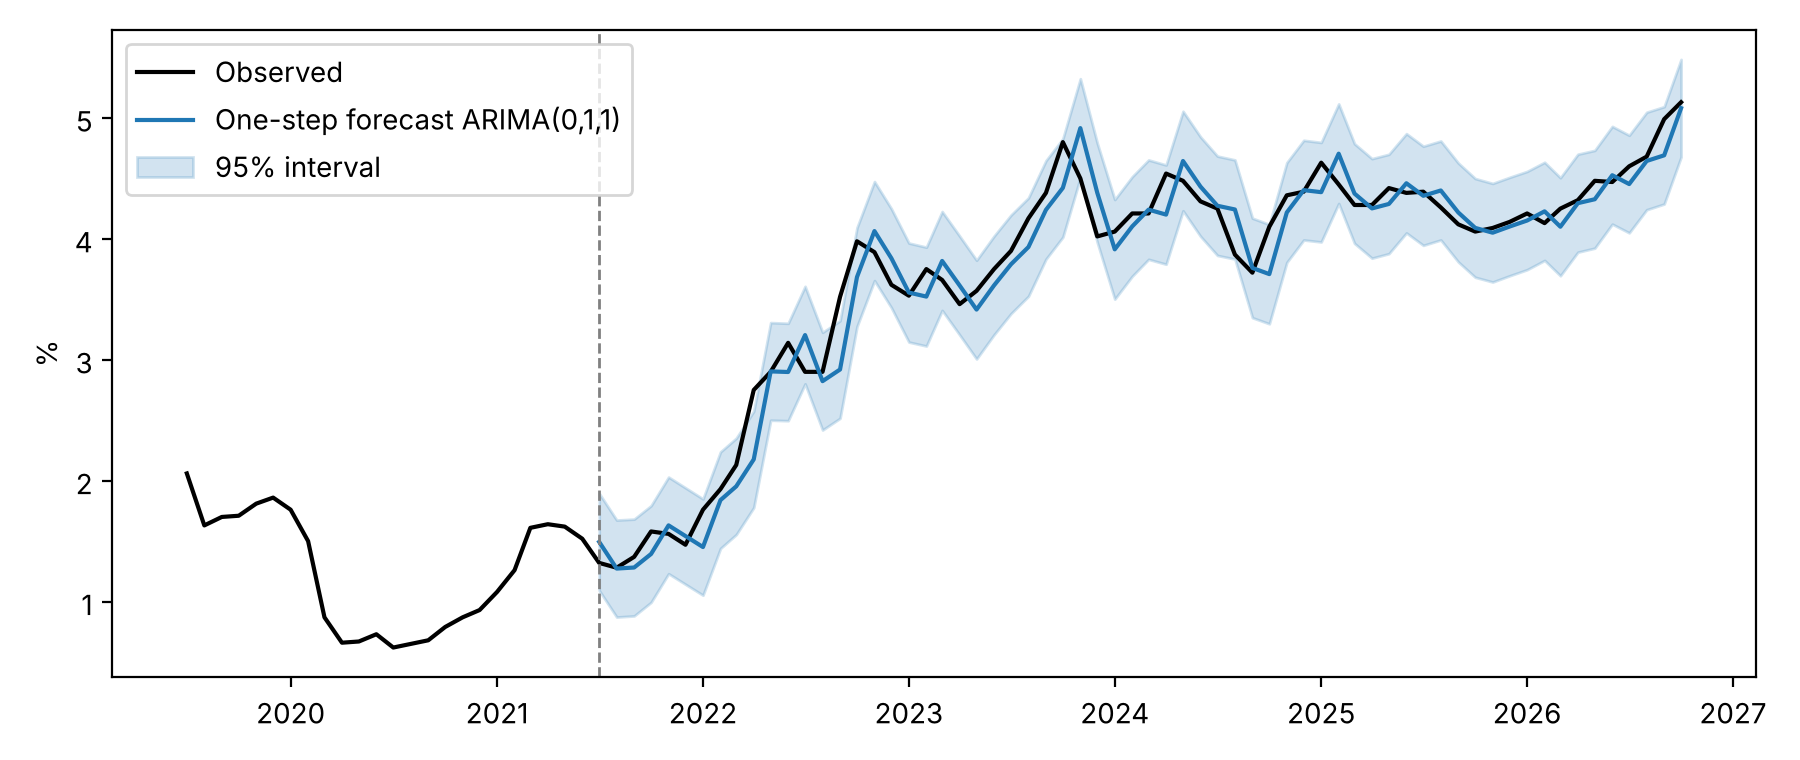
\includegraphics[width=0.85\textwidth]{out_of_sample.png}
\caption{One-step-ahead out-of-sample forecasts with 95\% intervals.}
\end{figure}

\subsection{Twelve-month forecast}

With the model estimated on the full sample the forecast is recursive: future shocks are set to zero and past shocks are replaced by the residuals. For an ARIMA(0,\,1,\,1) without drift
\begin{equation}
\hat y_{T+1} = y_T + \hat\theta\,\hat\varepsilon_T, \qquad \hat y_{T+h} = \hat y_{T+1} \quad (h \ge 2).
\end{equation}
Summing the errors of the future changes, every shock $\varepsilon_{T+j}$ with $j < h$ enters with weight $1 + \theta$ (once in its own month and $\theta$ times in the next one), except the last, which enters with weight 1:
\begin{equation}
\mathrm{Var}(e_{T+h}) = \sigma^2\left[1 + (h-1)(1+\theta)^2\right],
\end{equation}
which grows without bound, as for any series with a unit root.

\begin{table}[H]
\centering
\begin{tabular}{lcccc}
\toprule
Month & $h$ & Forecast (\%) & Std.\ error & 95\% interval \\
\midrule
November 2026 & 1 & 5.145 & 0.205 & [4.74,\ 5.55] \\
December 2026 & 2 & 5.145 & 0.338 & [4.48,\ 5.81] \\
January 2027 & 3 & 5.145 & 0.431 & [4.30,\ 5.99] \\
April 2027 & 6 & 5.145 & 0.634 & [3.90,\ 6.39] \\
October 2027 & 12 & 5.145 & 0.913 & [3.36,\ 6.93] \\
\bottomrule
\end{tabular}
\caption{Forecasts from the model estimated on the full sample.}
\end{table}

\begin{figure}[H]
\centering
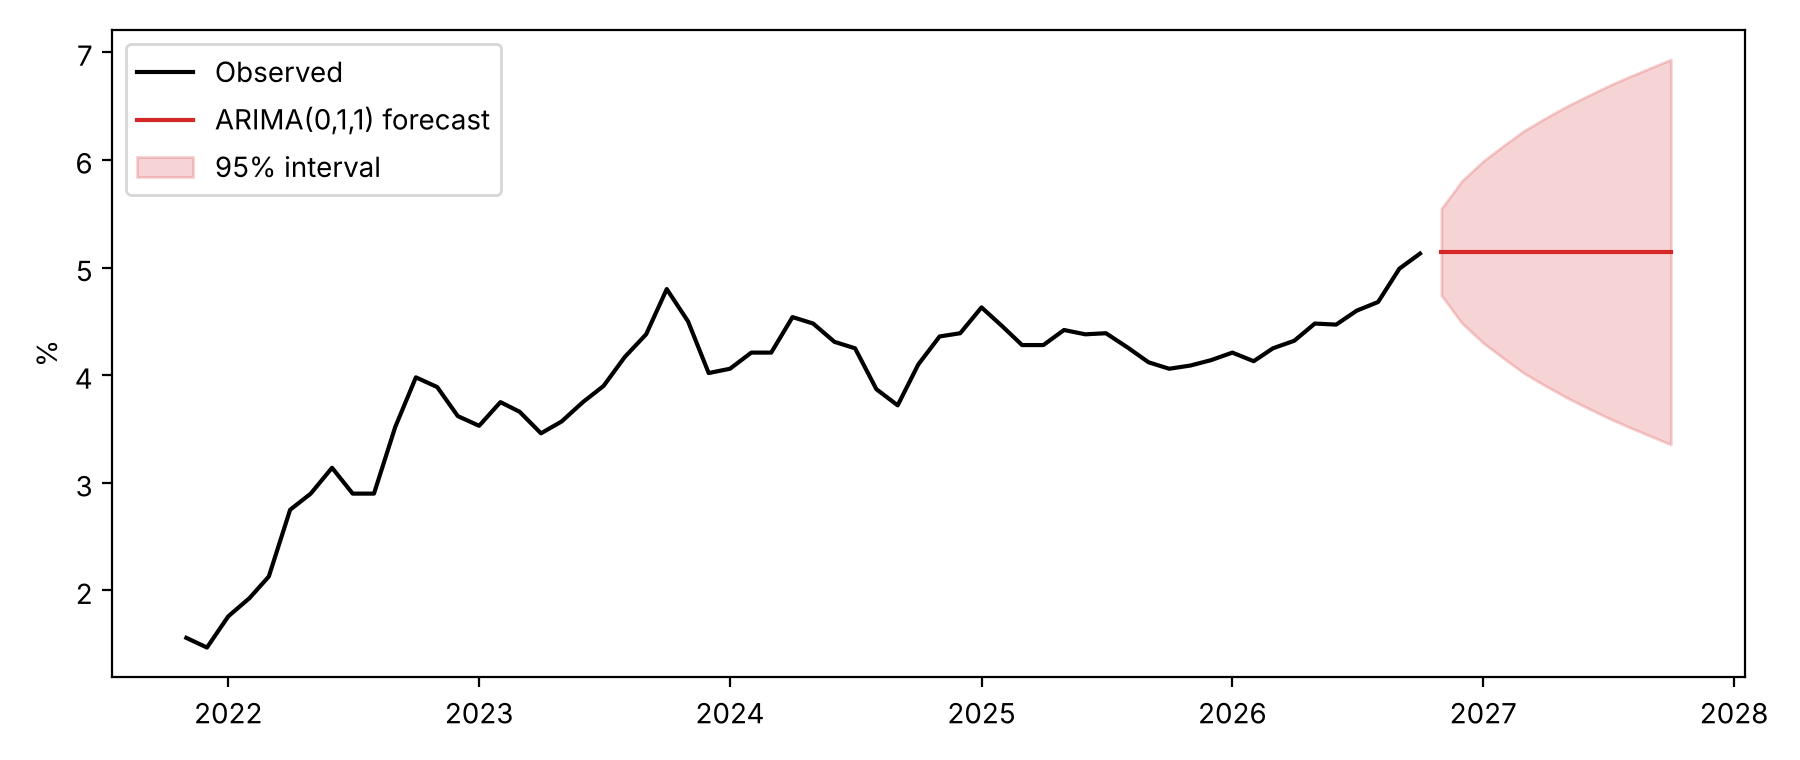
\includegraphics[width=0.85\textwidth]{forecast.png}
\caption{Twelve-month forecast with 95\% interval.}
\end{figure}

The forecast lies slightly above the last observation (5.13\%), because the last estimated shock is positive ($\hat\varepsilon_T = 0.049$) and $\hat\theta$ passes part of it on to the next month; afterwards it stays flat. At one year the 95\% interval is about $\pm1.8$ points wide: with a unit root and no drift, almost all the information useful to forecast the level is in the last observed value.

%======================================================================
\section{Double check with statsmodels}\label{sec:check}

To rule out implementation errors in our code, we recomputed the same quantities with the Python library \texttt{statsmodels} (functions \texttt{adfuller}, \texttt{kpss}, \texttt{acorr\_ljungbox}, \texttt{jarque\_bera} and the class \texttt{ARIMA}).

\begin{table}[H]
\centering
\begin{tabular}{lcc}
\toprule
Quantity & Our code & \texttt{statsmodels} \\
\midrule
ADF \texttt{'ct'} on $y_t$ & $-1.4528$ & $-1.4528$ \\
ADF \texttt{'c'} on $\Delta y_t$ & $-12.3636$ & $-12.3636$ \\
KPSS \texttt{'ct'} on $y_t$ & $0.8619$ & $0.8619$ \\
KPSS \texttt{'c'} on $\Delta y_t$ & $0.4200$ & $0.4200$ \\
Ljung--Box on $\Delta y_t$, $m=12$ & $27.4494$ & $27.4494$ \\
Jarque--Bera on $\Delta y_t$ & $83.1418$ & $83.1418$ \\
$\hat\theta$, ARIMA(0,\,1,\,1) & $0.3053$ & $0.2950$ \\
$SE(\hat\theta)$ & $0.0621$ & $0.0467$ \\
$\hat\sigma$ & $0.2054$ & $0.2051$ \\
Forecast, $h=1$ & $5.1448$ & $5.1453$ \\
Forecast SE, $h=12$ & $0.9128$ & $0.9045$ \\
\bottomrule
\end{tabular}
\caption{Our implementation versus \texttt{statsmodels}.}
\end{table}

\textbf{Findings.}
\begin{itemize}
\item \textbf{Test statistics} (ADF, KPSS, Ljung--Box, Jarque--Bera) coincide to the fourth decimal.
\item \textbf{ARIMA estimates.} \texttt{statsmodels} uses exact maximum likelihood, so $\hat\theta$ differs by about 0.01 (0.305 against 0.295). The Hannan--Rissanen standard error is larger because the second regression uses fewer observations and estimated shocks. The two estimators lead to the same conclusions, and the forecasts coincide to the third decimal.
\end{itemize}

The two independent implementations therefore agree, which validates the code used for the analysis.

%======================================================================
\section{Conclusions}

\begin{itemize}
\item GS10 is an interest rate, not a price: its changes in percentage points have a much more stable variance than its log-changes, so the model is built on the levels.
\item The ADF and KPSS tests agree that the yield has a unit root and that its monthly changes are stationary ($d = 1$); the drift is not significant.
\item The monthly changes are not white noise (Ljung--Box). ACF, PACF, AIC and BIC all point to an MA(1). Monthly averaging of a daily random walk generates exactly an MA(1) with $\theta = 2 - \sqrt3$, compatible with $\hat\theta = 0.305$.
\item $\theta$ is significant and stable, the model is invertible and the residuals show no autocorrelation; they have heavy tails, but the out-of-sample coverage of the 95\% intervals is close to 95\%.
\item Out of sample the ARIMA(0,\,1,\,1) beats the random walk by about 6\% in RMSE (one-sided Diebold--Mariano significant at 5\%) and beats the overfitted ARIMA(15,\,1,\,1).
\end{itemize}

\end{document}